\begin{ledgroupsized}[r]{120mm}
\footnotesize
\pstart
\noindent\textbf{Überlieferung:}
\pend
\end{ledgroupsized}
\begin{ledgroupsized}[r]{114mm}
\footnotesize
\pstart \parindent -6mm
\makebox[6mm][l]{\textit{L}}%
Aufzeichnung:
LH~XXXVII 5~Bl.~200.
Ein Blatt~2\textsuperscript{o};
Papiererhaltungsmaßnahmen;
alle Ränder beschnitten;
Blatt zweimal gefaltet.
Eine Seite auf Bl.~200~r\textsuperscript{o}; Bl.~200~v\textsuperscript{o} leer.
\pend
\end{ledgroupsized}
\vspace{5mm}
\begin{ledgroup}
\footnotesize
\pstart
\noindent%
\textbf{Datierungsgründe:}
Die vorliegende Aufzeichnung N.\;\ref{60362} untersucht den temporären
Verlust der Geschwindigkeiten zweier elastisch aufeinander stoßender Körper wegen \textendash\ und während \textendash\ der wechselseitigen Kompression.
Eins der Ergebnisse der Aufzeichnung ist die reziproke Proportion zwischen den Massen und den \textit{während der Kompression} eingebüßten Geschwindigkeiten
(\glqq dum se adhuc comprimunt\grqq, \refpassage{37_05_200_2a}{37_05_200_2b}).
Bei der Thematik von N.\;\ref{60362} allgemein und besonders bei der zitierten Formulierung 
lassen sich Übereinstimmungen mit einem weiteren diesem Thema gewidmeten Konzept (N.\;\ref{60358} in diesem Band) feststellen.
Dessen Schwerpunkt fasst dort Leibniz in einer Randanmerkung zusammen: 
\glqq Hic explicantur celeritates quae in corporibus duobus concurrentibus manent residuae, dum se urgent et ictu comprimunt\grqq\ (Anmerkung zu \refpassage{37_05_195_1a}{37_05_195_1b}).
\pend
\pstart
Mangels weiterer und aussagekräftigerer Anhaltspunkte für die Datierung des kurzen Textes wird für N.\;\ref{60362} die Datierung von N.\;\ref{60358} übernommen.
\pend 
\end{ledgroup}
\selectlanguage{latin}
\vspace{8mm}
\pstart
\noindent
\href{\Scan{LH_37_05_200r}}%
{\lbrack200~r\textsuperscript{o}\rbrack}
Si duo corpora 
\edtext{directe et centraliter}{\lemma{}\Bfootnote{directe et centraliter \textit{erg.~L}}} 
concurrant,\indexS{concursus directus et centralis duorum}
videndum
an in ipso concursu celeritates amissae%
\indexS{celeritas amissa}
sint molibus\indexS{moles}
\edlabel{37_05_200_1a}%
reciprocae.%
\edtext{}{%
\xxref{37_05_200_1a}{37_05_200_1b}%
\lemma{reciprocae.}\Bfootnote{%
\textit{(1)}~Ponantur corpora \textit{A} et \textit{B} concurr %
\textit{(2)}~Sit~\textit{L}}}%
\pend
\begin{edfigure}%
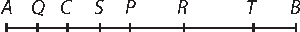
\includegraphics[scale=1]{gesamttex/edit_VIII-4/images/LH_37_05_200_d_200r.pdf} 
\edcaption{\lbrack\textit{Fig.~1}\rbrack}
\end{edfigure}
\pstart
Sit\edlabel{37_05_200_1b}
corporum \textit{A} et \textit{B} concurrentium
celeritatibus \textit{AP}, \textit{BP}
concursus%
\indexS{concursus}
in \textit{P}.
Sit eorundem corporum centrum\indexS{centrum gravitatis} \textit{C}. Ponamus moveri ea celeritatibus \textit{AC}, \textit{BC} in navi\indexS{navis} mota celeritate \textit{CP}. 
Et concurrentia in \textit{C} 
\edtext{amisisse unumquodque}{\lemma{amisisse}\Bfootnote{%
\textit{(1)}~partem %
\textit{(2)}~q %
\textit{(3)}~unumquodque~\textit{L}}} 
partem suae celeritatis; certum est celeritates
\edtext{in navi}{\lemma{}\Bfootnote{in navi \textit{erg.~L}}} 
amissas\indexS{celeritas amissa} esse reciproce proportionales, 
seu si \textit{A}, amiserit celeritatem \textit{AQ}; 
\textit{B} amisisse celeritatem \textit{BR}, et fore \textit{AQ} ad \textit{BR} ut \textit{B} ad \textit{A}. Residuaeque celeritates\indexS{celeritas residua} in navi erunt \textit{QC}, \textit{RC}. 
Sed cum spectando extra navim\indexS{navis} residuae celeritates sint \textit{QP} et 
\edtext{\textit{RP}\lbrack;\rbrack\ fuerint}{\lemma{\textit{RP}}\Bfootnote{%
\textit{(1)}~patet easdem esse amissas sive in navi spectes sive extra n %
\textit{(2)}~fuerint~\textit{L}}} 
autem primae \textit{AP}, \textit{BP}, patet easdem esse amissas \textit{AQ}, \textit{BR}; 
sive in navi\indexS{navis} spectes, sive extra navim;\indexS{navis} 
et cum in navi amissae sint reciprocae corporibus; 
\edlabel{37_05_200_2a}%
absolute dicendum est in corporum concursu\indexS{concursus corporum} 
\edtext{dum sese adhuc comprimunt}{\lemma{}\Bfootnote{dum sese adhuc comprimunt \textit{erg.~L}}}
celeritates amissas\indexS{celeritas amissa} esse corporibus reciproce proportionales.\indexS{celeritates corporibus reciproce proportionales}%
\edlabel{37_05_200_2b}
\pend 
\pstart 
Vicissim in corporum concursu,\indexS{concursus corporum} dum sese restituendo a se invicem rursus 
\edtext{recedunt, videndum an celeritates recuperatae\indexS{celeritas recuperata} sint}{%
\lemma{recedunt,}%
\Bfootnote{%
\textit{(1)}~celeritates recuperatae sunt %
\textit{(2)}~videndum an celeritates recuperatae sint~\textit{L}}}
corporibus reciproce proportionales.\indexS{celeritates corporibus reciproce proportionales} Redeamus ad 
\edtext{navim,\indexS{navis} quae}{\lemma{navim,}\Bfootnote{%
\textit{(1)}~et ponamus cor %
\textit{(2)}~quae~\textit{L}}} 
fertur celeritate \textit{CP}, et ponamus in ea 
\edtext{corpora post}{\lemma{corpora}\Bfootnote{%
\textit{(1)}~recuperasse %
\textit{(2)}~post~\textit{L}}}
ictum a se recedentia recuperasse
\edtext{\textit{A} celeritatem et directionem \textit{CQ}}{\lemma{\textit{A} celeritatem}\Bfootnote{%
\textit{(1)}~\textit{CQ}, %
\textit{(2)}~et directionem \textit{CQ}~\textit{L}}} 
et 
\edtext{\textit{B} celeritatem et directionem \textit{CR}; sumatur a \textit{P} versus \textit{A},}{%
\lemma{\textit{B}}%
\Bfootnote{celeritatem 
\bars{et directionem \textit{erg.}}
\textit{CR};
\textit{(1)}~manifestum est, spectanti ex %
\textit{(2)}~utique spectanti ex ripa %
\textit{(3)}~sumatur in \textit{CP} %
\textit{(4)}~sumatur a \textit{P} %
\textit{(a)}~retro %
\textit{(b)}~versus \textit{A},~\textit{L}}} 
ipsa \textit{PS} aequalis ipsi \textit{CQ}\lbrack,\rbrack\ erit \textit{CS} celeritas quam corpus \textit{A} 
\edtext{ex ripa\indexS{ripa}}{\lemma{ex}\Bfootnote{%
\textit{(1)}~navi %
\textit{(2)}~ripa~\textit{L}}} 
spectanti apparebit habere in \textit{P}. Similiter
\edtext{a \textit{P} versus}{\lemma{a \textit{P}}\Bfootnote{%
\textit{(1)}~antrorsum %
\textit{(2)}~versus~\textit{L}}} 
\textit{B} 
\edtext{sumatur \textit{PT}}{\lemma{sumatur}\Bfootnote{%
\textit{(1)}~\textit{PR} %
\textit{(2)}~\textit{PT}~\textit{L}}} 
aequalis ipsi 
\edtext{\textit{CR} et erit \textit{PT} celeritas quam}{\lemma{\textit{CR}}\Bfootnote{%
\textit{(1)}~et %
\textit{(2)}~et erit \textit{PT} celeritas quam~\textit{L}}} 
corpus \textit{B} ex ripa spectanti\indexS{spectans e ripa} 
apparebit habere in \textit{P}. Patet \textit{PS} esse
\edtext{$CP-CQ$, et \textit{PT}}{\lemma{$CP-CQ$, et}\Bfootnote{%
\textit{(1)}~\textit{PR} %
\textit{(2)}~\textit{PT}~\textit{L}}} 
esse $CP+CR$. Sed cum \textit{CQ} et \textit{CR} sint ut \textit{B} et \textit{A}, 
patet non posse $CP-CQ$ et $CP+CR$ ut \textit{B} et \textit{A}. 
\edtext{Itaque dici}{\lemma{Itaque}\Bfootnote{%
\textit{(1)}~fieri %
\textit{(2)}~dici~\textit{L}}} 
non potest celeritates recuperatas,\indexS{celeritas recuperata} spectando absolute seu extra \indexS{navis}navim\lbrack,\rbrack\ esse corporibus reciproce proportionales.\indexS{celeritates corporibus reciproce proportionales}
Sed celeritates retrorsum adhuc 
\edtext{acquirendae\indexS{celeritas acquirenda} sunt}{\lemma{acquirendae}\Bfootnote{%
\textit{(1)}~ab \textit{A} %
\textit{(a)}~sun %
\textit{(b)}~est %
\textit{(2)}~sunt~\textit{L}}} 
\textit{AQ} pro \textit{A}, et \textit{BR} pro 
\edtext{\textit{B}, sive}{\lemma{\textit{B},}\Bfootnote{%
\textit{(1)}~quae revera sun %
\textit{(2)}~sive~\textit{L}}} 
extra navim\indexS{navis} spectes sive in navi.\indexS{navis}
\pend
\pstart
Regula ergo haec est: 
\textls{celeritates ad seinvicem accedendi}\indexS{celeritates ad seinvicem accedendi}
\edtext{\textls{amissae\indexS{celeritas amissa} aut a}}{%
\lemma{\textls{amissae}}%
\Bfootnote{%
\textit{(1)}~\textls{et a} %
\textit{(2)}~aut %
\textit{(3)}~aut %
\textit{(4)}~\textls{aut a}~\textit{L}}}
\textls{se invicem recedendi\indexS{celeritates a seinvicem recedendi} recuperandae\indexS{celeritas recuperanda} sunt corporibus reciproce proportionales}.
\pend
